\documentclass[16pt]{beamer}

\usepackage[utf8]{inputenc}
\usepackage[main=russian, english]{babel}
\usetheme{Warsaw}
\usepackage{tikz}
\usepackage{adjustbox}

\title[Выпускная квалификационная работа]
        {О задаче целевого управления по результатам наблюдений, поступающих с запаздыванием}
\author[К. Ю. Егоров]
        {студент 4 курса К. Ю. Егоров\\
        научный руководитель --- к.ф-м.н., доцент И. В. Востриков}
\institute{Кафедра системного анализа}
\date{7 мая 2020 г.}

\begin{document}
        \maketitle
%%%%%%%%%%%%%%%%%%%%%%%%%%%%%%%%%%%%%%%%%%%%%%%%%%%%%%%%%%%%%%%%%%%%%%%%%%%%%%%%
        \begin{frame}[t]{Общая постановка задачи}
                \centering
                \begin{adjustbox}{max totalsize={0.9\textwidth}{.7\textheight}, center}
        \tikzset{every picture/.style={line width=0.75pt}}
        \begin{tikzpicture}[x=0.75pt,y=0.75pt,yscale=-1,xscale=1]
                %uncomment if require: \path (0,300); %set diagram left start at 0, and has height of 300

                %Shape: Rectangle [id:dp49899220246604004] 
                \draw  [fill={rgb, 255:red, 0; green, 0; blue, 0 }  ,fill opacity=1 ] (70,180) -- (140,180) -- (140,230) -- (70,230) -- cycle ;
                %Shape: Rectangle [id:dp5036156977339801] 
                \draw  [fill={rgb, 255:red, 0; green, 0; blue, 0 }  ,fill opacity=1 ] (70,240) -- (140,240) -- (140,250) -- (70,250) -- cycle ;
                %Shape: Circle [id:dp8783058595446472] 
                \draw  [fill={rgb, 255:red, 0; green, 0; blue, 0 }  ,fill opacity=1 ] (310,55) .. controls (310,46.72) and (316.72,40) .. (325,40) .. controls (333.28,40) and (340,46.72) .. (340,55) .. controls (340,63.28) and (333.28,70) .. (325,70) .. controls (316.72,70) and (310,63.28) .. (310,55) -- cycle ;
                %Curve Lines [id:da2875956857096633] 
                \draw    (319.6,56) .. controls (359.2,26.3) and (370.77,108.72) .. (426.5,96.4) ;
                \draw [shift={(428.2,96)}, rotate = 525.87] [color={rgb, 255:red, 0; green, 0; blue, 0 }  ][line width=0.75]    (10.93,-3.29) .. controls (6.95,-1.4) and (3.31,-0.3) .. (0,0) .. controls (3.31,0.3) and (6.95,1.4) .. (10.93,3.29)   ;
                %Curve Lines [id:da4933081009052841] 
                \draw  [dash pattern={on 4.5pt off 4.5pt}]  (293,48) .. controls (215.39,34.47) and (126.69,56.58) .. (123.84,164.37) ;
                \draw [shift={(123.8,166)}, rotate = 271.05] [color={rgb, 255:red, 0; green, 0; blue, 0 }  ][line width=0.75]    (10.93,-3.29) .. controls (6.95,-1.4) and (3.31,-0.3) .. (0,0) .. controls (3.31,0.3) and (6.95,1.4) .. (10.93,3.29)   ;
                %Curve Lines [id:da11306010539930555] 
                \draw  [dash pattern={on 4.5pt off 4.5pt}]  (156.6,191.2) .. controls (265.5,190.8) and (311.67,136.7) .. (314.91,79.73) ;
                \draw [shift={(315,78)}, rotate = 452.39] [color={rgb, 255:red, 0; green, 0; blue, 0 }  ][line width=0.75]    (10.93,-3.29) .. controls (6.95,-1.4) and (3.31,-0.3) .. (0,0) .. controls (3.31,0.3) and (6.95,1.4) .. (10.93,3.29)   ;

                % Text Node
                \draw (430.8,88.4) node [anchor=north west][inner sep=0.75pt]    {$\frac{dx}{dt} = A(t)x + B(t)v$};
                % Text Node
                \draw (88.8,44.4) node [anchor=north west][inner sep=0.75pt]    {$x( t-h_{\mathrm{tc}})$};
                % Text Node
                \draw (360, 4) node [anchor=north west][inner sep=0.75pt]   [align=left] {Управляемый объект};
                % Text Node
                \draw (150, 210) node [anchor=north west][inner sep=0.75pt]   [align=left] {Центр управления};
                % Text Node
                \draw (292.8,152.4) node [anchor=north west][inner sep=0.75pt]    {$v( t-h_{\mathrm{fc}})$};
                % Text Node
                \draw (150,230) node [anchor=north west][inner sep=0.75pt]  [font=\small] [align=left] {\textit{{\small Получает данные о состоянии}}};
                % Text Node
                \draw (360, 24) node [anchor=north west][inner sep=0.75pt]  [font=\small] [align=left] {{\small \textit{Получает управление }}\\};
                % Text Node
                \draw (360, 38) node [anchor=north west][inner sep=0.75pt]  [font=\small] [align=left] {{\small \textit{из центра с запаздыванием}}};
                % Text Node
                \draw (150, 242) node [anchor=north west][inner sep=0.75pt]  [font=\small] [align=left] {\textit{{\small объекта с запаздыванием}}};
        \end{tikzpicture}
\end{adjustbox}
                \vspace{0.5cm}
                \begin{equation*}
                        \begin{aligned}
                                \dot x = A(t)x + B(t)u, \qquad\mbox{где }
                                &u(t) = u(t,\,x(t - h)) = v(t + h_{\mathrm{fc}}),\\
                                &h = h_{\mathrm{tc}} + h_{\mathrm{fc}}.
                        \end{aligned}
                \end{equation*}
        \end{frame}
       \begin{frame}{Непрерывная линейно-квадратичная задача}
                Рассмотрим задачу
                $
                        \dot x = A(t)x+B(t)u,
                $
                $
                        J(u)
                =
                        \int_{t_0}^{t_1}
                [
                \langle
                x,\,M(s)x
                \rangle
                +
                \langle
                u,\,N(s)u
                \rangle
                ]\,ds
                        +
                        \langle
                        x(t_1),\,Tx(t_1)
                        \rangle
                \to
                        \min\limits_{u},
                $
где $M(s) = M^{\mathrm{T}}(s) \geqslant 0$,
$N(s) = N^{\mathrm{T}}(s) > 0$,
$T = T^{\mathrm{T}} > 0$.
                \vspace{1cm}

                Введём функцию цены
                $
                        V(t_0, x_0) = \inf_{u}{J(u)}
                $ и будем искать её в виде $V(t,x) = \langle x, P(t) x\rangle$, где $P(t) = P^{\mathrm{T}}(t) > 0.$

                \vspace{1cm}

                Функция цены удолетворяет уравнению Гамильтона--Якоби--Беллмана:
                \begin{equation*}
\begin{cases}
        \frac{\partial V}{\partial t}
        +
        \min\limits_{u}
        \left\{
        
\left\langle
\frac{\partial V}{\partial x}
,\,
Ax + Bu
\right\rangle
+
\langle
x,\,Mx
\rangle
+
\langle
u,\,Nu
\rangle
        
        \right\}
        =
        0,
\\
        V(t_1,\,x)
        =
        \langle x,\,Tx \rangle.
\end{cases}
\end{equation*}
        \end{frame}
        \begin{frame}{Непрерывная линейно-квадратичная задача}
                Решив уравнение Гамильтона--Якоби--Беллмана, получим
                \begin{equation*}
                        u^*(t) = -N^{-1}(t)B^{\mathrm{T}}(t) P(t)x(t),
                \end{equation*}
                где $P(t)$ удовлетворяет уравнению Риккати:
                \begin{equation*}
                        \begin{cases}
                                \dot P + PA + A^{\mathrm{T}} P - PBN^{-1}B^{\mathrm{T}} P + M = 0,\\
                                P(t_1) = T,
                        \end{cases}
                \end{equation*}
                а $x(t)$ --- текущее состояние объекта, которое можно вычислить таким образом:
                \begin{equation*}
                        x(t) =
                        \begin{cases}
                                X(t,t_0)x_0 + \int\limits_{t_0}^{t}X(t,s)B(s)u^*(s)\,ds,
                                &
                                t \in [t_0,t_0 + h],
                                \\
                                X(t,t - h)x(t-h) + \int\limits_{t - h}^{t}X(t,s)B(s)u^*(s)\,ds,
                                &
                                t \in (t_0 + h,t_1].
                        \end{cases}
                \end{equation*}
        \end{frame}
%%%%%%%%%%%%%%%%%%%%%%%%%%%%%%%%%%%%%%%%%%%%%%%%%%%%%%%%%%%%%%%%%%%%%%%%%%%%%%%%
        \begin{frame}[t]{Переход к дискретной системе}
                \centering
                

\tikzset{every picture/.style={line width=0.75pt}} %set default line width to 0.75pt        

\begin{tikzpicture}[x=0.75pt,y=0.75pt,yscale=-1,xscale=1]
%uncomment if require: \path (0,300); %set diagram left start at 0, and has height of 300

%Straight Lines [id:da3371936483919118] 
\draw    (10,90) -- (368,90) ;
\draw [shift={(370,90)}, rotate = 180] [color={rgb, 255:red, 0; green, 0; blue, 0 }  ][line width=0.75]    (10.93,-3.29) .. controls (6.95,-1.4) and (3.31,-0.3) .. (0,0) .. controls (3.31,0.3) and (6.95,1.4) .. (10.93,3.29)   ;
%Straight Lines [id:da7871764172333664] 
\draw    (40,50) -- (40,88) ;
\draw [shift={(40,90)}, rotate = 270] [color={rgb, 255:red, 0; green, 0; blue, 0 }  ][line width=0.75]    (10.93,-3.29) .. controls (6.95,-1.4) and (3.31,-0.3) .. (0,0) .. controls (3.31,0.3) and (6.95,1.4) .. (10.93,3.29)   ;
%Straight Lines [id:da5441997885317058] 
\draw    (120,70) -- (120,88) ;
\draw [shift={(120,90)}, rotate = 270] [color={rgb, 255:red, 0; green, 0; blue, 0 }  ][line width=0.75]    (10.93,-3.29) .. controls (6.95,-1.4) and (3.31,-0.3) .. (0,0) .. controls (3.31,0.3) and (6.95,1.4) .. (10.93,3.29)   ;
%Straight Lines [id:da36707750473745593] 
\draw    (200,70) -- (200,88) ;
\draw [shift={(200,90)}, rotate = 270] [color={rgb, 255:red, 0; green, 0; blue, 0 }  ][line width=0.75]    (10.93,-3.29) .. controls (6.95,-1.4) and (3.31,-0.3) .. (0,0) .. controls (3.31,0.3) and (6.95,1.4) .. (10.93,3.29)   ;
%Straight Lines [id:da16240341438550177] 
\draw    (280,70) -- (280,88) ;
\draw [shift={(280,90)}, rotate = 270] [color={rgb, 255:red, 0; green, 0; blue, 0 }  ][line width=0.75]    (10.93,-3.29) .. controls (6.95,-1.4) and (3.31,-0.3) .. (0,0) .. controls (3.31,0.3) and (6.95,1.4) .. (10.93,3.29)   ;
%Curve Lines [id:da1851824806305855] 
\draw    (40,90) .. controls (70.29,1.69) and (226.24,0.42) .. (259.04,87.34) ;
\draw [shift={(260,90)}, rotate = 251.14] [fill={rgb, 255:red, 0; green, 0; blue, 0 }  ][line width=0.08]  [draw opacity=0] (10.72,-5.15) -- (0,0) -- (10.72,5.15) -- (7.12,0) -- cycle    ;
%Straight Lines [id:da5796770396576605] 
\draw  [dash pattern={on 4.5pt off 4.5pt}]  (260,90) -- (260,160) ;
%Straight Lines [id:da7576783972344275] 
\draw  [dash pattern={on 4.5pt off 4.5pt}]  (340,90) -- (340,160) ;
%Straight Lines [id:da7144770541416994] 
\draw    (260,108.5) .. controls (261.67,106.83) and (263.33,106.83) .. (265,108.5) .. controls (266.67,110.17) and (268.33,110.17) .. (270,108.5) .. controls (271.67,106.83) and (273.33,106.83) .. (275,108.5) .. controls (276.67,110.17) and (278.33,110.17) .. (280,108.5) .. controls (281.67,106.83) and (283.33,106.83) .. (285,108.5) .. controls (286.67,110.17) and (288.33,110.17) .. (290,108.5) .. controls (291.67,106.83) and (293.33,106.83) .. (295,108.5) .. controls (296.67,110.17) and (298.33,110.17) .. (300,108.5) .. controls (301.67,106.83) and (303.33,106.83) .. (305,108.5) .. controls (306.67,110.17) and (308.33,110.17) .. (310,108.5) .. controls (311.67,106.83) and (313.33,106.83) .. (315,108.5) .. controls (316.67,110.17) and (318.33,110.17) .. (320,108.5) .. controls (321.67,106.83) and (323.33,106.83) .. (325,108.5) .. controls (326.67,110.17) and (328.33,110.17) .. (330,108.5) .. controls (331.67,106.83) and (333.33,106.83) .. (335,108.5) .. controls (336.67,110.17) and (338.33,110.17) .. (340,108.5) -- (340,108.5)(260,111.5) .. controls (261.67,109.83) and (263.33,109.83) .. (265,111.5) .. controls (266.67,113.17) and (268.33,113.17) .. (270,111.5) .. controls (271.67,109.83) and (273.33,109.83) .. (275,111.5) .. controls (276.67,113.17) and (278.33,113.17) .. (280,111.5) .. controls (281.67,109.83) and (283.33,109.83) .. (285,111.5) .. controls (286.67,113.17) and (288.33,113.17) .. (290,111.5) .. controls (291.67,109.83) and (293.33,109.83) .. (295,111.5) .. controls (296.67,113.17) and (298.33,113.17) .. (300,111.5) .. controls (301.67,109.83) and (303.33,109.83) .. (305,111.5) .. controls (306.67,113.17) and (308.33,113.17) .. (310,111.5) .. controls (311.67,109.83) and (313.33,109.83) .. (315,111.5) .. controls (316.67,113.17) and (318.33,113.17) .. (320,111.5) .. controls (321.67,109.83) and (323.33,109.83) .. (325,111.5) .. controls (326.67,113.17) and (328.33,113.17) .. (330,111.5) .. controls (331.67,109.83) and (333.33,109.83) .. (335,111.5) .. controls (336.67,113.17) and (338.33,113.17) .. (340,111.5) -- (340,111.5) ;
%Straight Lines [id:da8940007297109899] 
\draw [color={rgb, 255:red, 255; green, 255; blue, 255 }  ,draw opacity=1 ]   (0,0) -- (390,0) ;
%Straight Lines [id:da5623278208635653] 
\draw  [dash pattern={on 4.5pt off 4.5pt}]  (180,90) -- (180,160) ;
%Straight Lines [id:da8394004330187886] 
\draw  [dash pattern={on 4.5pt off 4.5pt}]  (20,90) -- (20,160) ;
%Straight Lines [id:da2531293148410282] 
\draw  [dash pattern={on 4.5pt off 4.5pt}]  (100,90) -- (100,160) ;
%Straight Lines [id:da4084203199337314] 
\draw    (180,118.5) .. controls (181.67,116.83) and (183.33,116.83) .. (185,118.5) .. controls (186.67,120.17) and (188.33,120.17) .. (190,118.5) .. controls (191.67,116.83) and (193.33,116.83) .. (195,118.5) .. controls (196.67,120.17) and (198.33,120.17) .. (200,118.5) .. controls (201.67,116.83) and (203.33,116.83) .. (205,118.5) .. controls (206.67,120.17) and (208.33,120.17) .. (210,118.5) .. controls (211.67,116.83) and (213.33,116.83) .. (215,118.5) .. controls (216.67,120.17) and (218.33,120.17) .. (220,118.5) .. controls (221.67,116.83) and (223.33,116.83) .. (225,118.5) .. controls (226.67,120.17) and (228.33,120.17) .. (230,118.5) .. controls (231.67,116.83) and (233.33,116.83) .. (235,118.5) .. controls (236.67,120.17) and (238.33,120.17) .. (240,118.5) .. controls (241.67,116.83) and (243.33,116.83) .. (245,118.5) .. controls (246.67,120.17) and (248.33,120.17) .. (250,118.5) .. controls (251.67,116.83) and (253.33,116.83) .. (255,118.5) .. controls (256.67,120.17) and (258.33,120.17) .. (260,118.5) -- (260,118.5)(180,121.5) .. controls (181.67,119.83) and (183.33,119.83) .. (185,121.5) .. controls (186.67,123.17) and (188.33,123.17) .. (190,121.5) .. controls (191.67,119.83) and (193.33,119.83) .. (195,121.5) .. controls (196.67,123.17) and (198.33,123.17) .. (200,121.5) .. controls (201.67,119.83) and (203.33,119.83) .. (205,121.5) .. controls (206.67,123.17) and (208.33,123.17) .. (210,121.5) .. controls (211.67,119.83) and (213.33,119.83) .. (215,121.5) .. controls (216.67,123.17) and (218.33,123.17) .. (220,121.5) .. controls (221.67,119.83) and (223.33,119.83) .. (225,121.5) .. controls (226.67,123.17) and (228.33,123.17) .. (230,121.5) .. controls (231.67,119.83) and (233.33,119.83) .. (235,121.5) .. controls (236.67,123.17) and (238.33,123.17) .. (240,121.5) .. controls (241.67,119.83) and (243.33,119.83) .. (245,121.5) .. controls (246.67,123.17) and (248.33,123.17) .. (250,121.5) .. controls (251.67,119.83) and (253.33,119.83) .. (255,121.5) .. controls (256.67,123.17) and (258.33,123.17) .. (260,121.5) -- (260,121.5) ;
%Straight Lines [id:da9815095577419825] 
\draw    (100,128.5) .. controls (101.67,126.83) and (103.33,126.83) .. (105,128.5) .. controls (106.67,130.17) and (108.33,130.17) .. (110,128.5) .. controls (111.67,126.83) and (113.33,126.83) .. (115,128.5) .. controls (116.67,130.17) and (118.33,130.17) .. (120,128.5) .. controls (121.67,126.83) and (123.33,126.83) .. (125,128.5) .. controls (126.67,130.17) and (128.33,130.17) .. (130,128.5) .. controls (131.67,126.83) and (133.33,126.83) .. (135,128.5) .. controls (136.67,130.17) and (138.33,130.17) .. (140,128.5) .. controls (141.67,126.83) and (143.33,126.83) .. (145,128.5) .. controls (146.67,130.17) and (148.33,130.17) .. (150,128.5) .. controls (151.67,126.83) and (153.33,126.83) .. (155,128.5) .. controls (156.67,130.17) and (158.33,130.17) .. (160,128.5) .. controls (161.67,126.83) and (163.33,126.83) .. (165,128.5) .. controls (166.67,130.17) and (168.33,130.17) .. (170,128.5) .. controls (171.67,126.83) and (173.33,126.83) .. (175,128.5) .. controls (176.67,130.17) and (178.33,130.17) .. (180,128.5) -- (180,128.5)(100,131.5) .. controls (101.67,129.83) and (103.33,129.83) .. (105,131.5) .. controls (106.67,133.17) and (108.33,133.17) .. (110,131.5) .. controls (111.67,129.83) and (113.33,129.83) .. (115,131.5) .. controls (116.67,133.17) and (118.33,133.17) .. (120,131.5) .. controls (121.67,129.83) and (123.33,129.83) .. (125,131.5) .. controls (126.67,133.17) and (128.33,133.17) .. (130,131.5) .. controls (131.67,129.83) and (133.33,129.83) .. (135,131.5) .. controls (136.67,133.17) and (138.33,133.17) .. (140,131.5) .. controls (141.67,129.83) and (143.33,129.83) .. (145,131.5) .. controls (146.67,133.17) and (148.33,133.17) .. (150,131.5) .. controls (151.67,129.83) and (153.33,129.83) .. (155,131.5) .. controls (156.67,133.17) and (158.33,133.17) .. (160,131.5) .. controls (161.67,129.83) and (163.33,129.83) .. (165,131.5) .. controls (166.67,133.17) and (168.33,133.17) .. (170,131.5) .. controls (171.67,129.83) and (173.33,129.83) .. (175,131.5) .. controls (176.67,133.17) and (178.33,133.17) .. (180,131.5) -- (180,131.5) ;
%Straight Lines [id:da2015294166480902] 
\draw    (20,98.5) .. controls (21.67,96.83) and (23.33,96.83) .. (25,98.5) .. controls (26.67,100.17) and (28.33,100.17) .. (30,98.5) .. controls (31.67,96.83) and (33.33,96.83) .. (35,98.5) .. controls (36.67,100.17) and (38.33,100.17) .. (40,98.5) .. controls (41.67,96.83) and (43.33,96.83) .. (45,98.5) .. controls (46.67,100.17) and (48.33,100.17) .. (50,98.5) .. controls (51.67,96.83) and (53.33,96.83) .. (55,98.5) .. controls (56.67,100.17) and (58.33,100.17) .. (60,98.5) .. controls (61.67,96.83) and (63.33,96.83) .. (65,98.5) .. controls (66.67,100.17) and (68.33,100.17) .. (70,98.5) .. controls (71.67,96.83) and (73.33,96.83) .. (75,98.5) .. controls (76.67,100.17) and (78.33,100.17) .. (80,98.5) .. controls (81.67,96.83) and (83.33,96.83) .. (85,98.5) .. controls (86.67,100.17) and (88.33,100.17) .. (90,98.5) .. controls (91.67,96.83) and (93.33,96.83) .. (95,98.5) .. controls (96.67,100.17) and (98.33,100.17) .. (100,98.5) -- (100,98.5)(20,101.5) .. controls (21.67,99.83) and (23.33,99.83) .. (25,101.5) .. controls (26.67,103.17) and (28.33,103.17) .. (30,101.5) .. controls (31.67,99.83) and (33.33,99.83) .. (35,101.5) .. controls (36.67,103.17) and (38.33,103.17) .. (40,101.5) .. controls (41.67,99.83) and (43.33,99.83) .. (45,101.5) .. controls (46.67,103.17) and (48.33,103.17) .. (50,101.5) .. controls (51.67,99.83) and (53.33,99.83) .. (55,101.5) .. controls (56.67,103.17) and (58.33,103.17) .. (60,101.5) .. controls (61.67,99.83) and (63.33,99.83) .. (65,101.5) .. controls (66.67,103.17) and (68.33,103.17) .. (70,101.5) .. controls (71.67,99.83) and (73.33,99.83) .. (75,101.5) .. controls (76.67,103.17) and (78.33,103.17) .. (80,101.5) .. controls (81.67,99.83) and (83.33,99.83) .. (85,101.5) .. controls (86.67,103.17) and (88.33,103.17) .. (90,101.5) .. controls (91.67,99.83) and (93.33,99.83) .. (95,101.5) .. controls (96.67,103.17) and (98.33,103.17) .. (100,101.5) -- (100,101.5) ;
%Straight Lines [id:da7866538445325351] 
\draw  [dash pattern={on 4.5pt off 4.5pt}]  (40,90) -- (40,160) ;
%Straight Lines [id:da8037148250929482] 
\draw    (41,150) -- (99,150) ;
\draw [shift={(98,150)}, rotate = 0] [fill={rgb, 255:red, 0; green, 0; blue, 0 }  ][line width=0.08]  [draw opacity=0] (8.93,-4.29) -- (0,0) -- (8.93,4.29) -- cycle    ;
\draw [shift={(42,150)}, rotate = 180] [fill={rgb, 255:red, 0; green, 0; blue, 0 }  ][line width=0.08]  [draw opacity=0] (8.93,-4.29) -- (0,0) -- (8.93,4.29) -- cycle    ;

% Text Node
\draw (377,82.4) node [anchor=north west][inner sep=0.75pt]    {$t$};
% Text Node
\draw (31,30.4) node [anchor=north west][inner sep=0.75pt]    {$x^{k}$};
% Text Node
\draw (111,50.4) node [anchor=north west][inner sep=0.75pt]    {$x^{k+1}$};
% Text Node
\draw (191,50.4) node [anchor=north west][inner sep=0.75pt]    {$x^{k+2}$};
% Text Node
\draw (11,52.4) node [anchor=north west][inner sep=0.75pt]    {$\dotsc $};
% Text Node
\draw (311,52.4) node [anchor=north west][inner sep=0.75pt]    {$\dotsc $};
% Text Node
\draw (271,50.4) node [anchor=north west][inner sep=0.75pt]    {$x^{k+3}$};
% Text Node
\draw (147,2.4) node [anchor=north west][inner sep=0.75pt]    {$h$};
% Text Node
\draw (291,112.4) node [anchor=north west][inner sep=0.75pt]    {$u^{k}$};
% Text Node
\draw (211,122.4) node [anchor=north west][inner sep=0.75pt]    {$u^{k-1}$};
% Text Node
\draw (131,132.4) node [anchor=north west][inner sep=0.75pt]    {$u^{k-2}$};
% Text Node
\draw (51,102.4) node [anchor=north west][inner sep=0.75pt]    {$u^{k-3}$};
% Text Node
\draw (61,152.4) node [anchor=north west][inner sep=0.75pt]    {$\hat{h}$};


\end{tikzpicture}

                \begin{equation*}
                        \boxed{
                                x^{k+1}
                                =
                                \Phi^k x^k + \Gamma_1^k u^{k-m} + \Gamma_2^k u^{k-m-1}
                        }
                \end{equation*}
                \begin{equation*}
                        \begin{aligned}
                                \Phi^k = X(t^{k+1},t^k), \quad
                                &\Gamma_1^k
                                =
                                \int_{t^{k} + \hat h}^{t^{k+1}} X(t^{k+1},s)B(s)\,ds,
                                \\
                                &\Gamma_2^k
                                =
                                \int_{t^k}^{t^{k} + \hat h} X(t^{k} + \hat h,s)B(s)\,ds.
                        \end{aligned}
                \end{equation*}
        \end{frame}

%%%%%%%%%%%%%%%%%%%%%%%%%%%%%%%%%%%%%%%%%%%%%%%%%%%%%%%%%%%%%%%%%%%%%%%%%%%%%%%%
        \begin{frame}[t]{Упрощение системы}
                \centering
                

\tikzset{every picture/.style={line width=0.75pt}} %set default line width to 0.75pt        

\begin{tikzpicture}[x=0.75pt,y=0.75pt,yscale=-1,xscale=1]
%uncomment if require: \path (0,300); %set diagram left start at 0, and has height of 300

%Straight Lines [id:da01928855054151435] 
\draw    (10,90) -- (368,90) ;
\draw [shift={(370,90)}, rotate = 180] [color={rgb, 255:red, 0; green, 0; blue, 0 }  ][line width=0.75]    (10.93,-3.29) .. controls (6.95,-1.4) and (3.31,-0.3) .. (0,0) .. controls (3.31,0.3) and (6.95,1.4) .. (10.93,3.29)   ;
%Straight Lines [id:da4146766554691299] 
\draw [color={rgb, 255:red, 65; green, 117; blue, 5 }  ,draw opacity=1 ]   (40,50) -- (40,88) ;
\draw [shift={(40,90)}, rotate = 270] [color={rgb, 255:red, 65; green, 117; blue, 5 }  ,draw opacity=1 ][line width=0.75]    (10.93,-3.29) .. controls (6.95,-1.4) and (3.31,-0.3) .. (0,0) .. controls (3.31,0.3) and (6.95,1.4) .. (10.93,3.29)   ;
%Straight Lines [id:da4624117459684317] 
\draw    (120,20) -- (120,88) ;
\draw [shift={(120,90)}, rotate = 270] [color={rgb, 255:red, 0; green, 0; blue, 0 }  ][line width=0.75]    (10.93,-3.29) .. controls (6.95,-1.4) and (3.31,-0.3) .. (0,0) .. controls (3.31,0.3) and (6.95,1.4) .. (10.93,3.29)   ;
%Straight Lines [id:da9441887002875778] 
\draw    (200,40) -- (200,88) ;
\draw [shift={(200,90)}, rotate = 270] [color={rgb, 255:red, 0; green, 0; blue, 0 }  ][line width=0.75]    (10.93,-3.29) .. controls (6.95,-1.4) and (3.31,-0.3) .. (0,0) .. controls (3.31,0.3) and (6.95,1.4) .. (10.93,3.29)   ;
%Straight Lines [id:da3602472791134742] 
\draw    (280,70) -- (280,88) ;
\draw [shift={(280,90)}, rotate = 270] [color={rgb, 255:red, 0; green, 0; blue, 0 }  ][line width=0.75]    (10.93,-3.29) .. controls (6.95,-1.4) and (3.31,-0.3) .. (0,0) .. controls (3.31,0.3) and (6.95,1.4) .. (10.93,3.29)   ;
%Straight Lines [id:da3053082735783992] 
\draw  [dash pattern={on 4.5pt off 4.5pt}]  (260,90) -- (260,160) ;
%Straight Lines [id:da16243227227702783] 
\draw  [dash pattern={on 4.5pt off 4.5pt}]  (340,90) -- (340,160) ;
%Straight Lines [id:da2927980241490754] 
\draw    (260,108.5) .. controls (261.67,106.83) and (263.33,106.83) .. (265,108.5) .. controls (266.67,110.17) and (268.33,110.17) .. (270,108.5) .. controls (271.67,106.83) and (273.33,106.83) .. (275,108.5) .. controls (276.67,110.17) and (278.33,110.17) .. (280,108.5) .. controls (281.67,106.83) and (283.33,106.83) .. (285,108.5) .. controls (286.67,110.17) and (288.33,110.17) .. (290,108.5) .. controls (291.67,106.83) and (293.33,106.83) .. (295,108.5) .. controls (296.67,110.17) and (298.33,110.17) .. (300,108.5) .. controls (301.67,106.83) and (303.33,106.83) .. (305,108.5) .. controls (306.67,110.17) and (308.33,110.17) .. (310,108.5) .. controls (311.67,106.83) and (313.33,106.83) .. (315,108.5) .. controls (316.67,110.17) and (318.33,110.17) .. (320,108.5) .. controls (321.67,106.83) and (323.33,106.83) .. (325,108.5) .. controls (326.67,110.17) and (328.33,110.17) .. (330,108.5) .. controls (331.67,106.83) and (333.33,106.83) .. (335,108.5) .. controls (336.67,110.17) and (338.33,110.17) .. (340,108.5) -- (340,108.5)(260,111.5) .. controls (261.67,109.83) and (263.33,109.83) .. (265,111.5) .. controls (266.67,113.17) and (268.33,113.17) .. (270,111.5) .. controls (271.67,109.83) and (273.33,109.83) .. (275,111.5) .. controls (276.67,113.17) and (278.33,113.17) .. (280,111.5) .. controls (281.67,109.83) and (283.33,109.83) .. (285,111.5) .. controls (286.67,113.17) and (288.33,113.17) .. (290,111.5) .. controls (291.67,109.83) and (293.33,109.83) .. (295,111.5) .. controls (296.67,113.17) and (298.33,113.17) .. (300,111.5) .. controls (301.67,109.83) and (303.33,109.83) .. (305,111.5) .. controls (306.67,113.17) and (308.33,113.17) .. (310,111.5) .. controls (311.67,109.83) and (313.33,109.83) .. (315,111.5) .. controls (316.67,113.17) and (318.33,113.17) .. (320,111.5) .. controls (321.67,109.83) and (323.33,109.83) .. (325,111.5) .. controls (326.67,113.17) and (328.33,113.17) .. (330,111.5) .. controls (331.67,109.83) and (333.33,109.83) .. (335,111.5) .. controls (336.67,113.17) and (338.33,113.17) .. (340,111.5) -- (340,111.5) ;
%Straight Lines [id:da7418650605563305] 
\draw [color={rgb, 255:red, 255; green, 255; blue, 255 }  ,draw opacity=1 ]   (0,0) -- (390,0) ;
%Straight Lines [id:da09218442968269502] 
\draw  [dash pattern={on 4.5pt off 4.5pt}]  (180,90) -- (180,160) ;
%Straight Lines [id:da902101020965036] 
\draw  [dash pattern={on 4.5pt off 4.5pt}]  (20,90) -- (20,160) ;
%Straight Lines [id:da8920476808059208] 
\draw  [dash pattern={on 4.5pt off 4.5pt}]  (100,90) -- (100,160) ;
%Straight Lines [id:da15222809490861489] 
\draw [color={rgb, 255:red, 65; green, 117; blue, 5 }  ,draw opacity=1 ]   (180,118.5) .. controls (181.67,116.83) and (183.33,116.83) .. (185,118.5) .. controls (186.67,120.17) and (188.33,120.17) .. (190,118.5) .. controls (191.67,116.83) and (193.33,116.83) .. (195,118.5) .. controls (196.67,120.17) and (198.33,120.17) .. (200,118.5) .. controls (201.67,116.83) and (203.33,116.83) .. (205,118.5) .. controls (206.67,120.17) and (208.33,120.17) .. (210,118.5) .. controls (211.67,116.83) and (213.33,116.83) .. (215,118.5) .. controls (216.67,120.17) and (218.33,120.17) .. (220,118.5) .. controls (221.67,116.83) and (223.33,116.83) .. (225,118.5) .. controls (226.67,120.17) and (228.33,120.17) .. (230,118.5) .. controls (231.67,116.83) and (233.33,116.83) .. (235,118.5) .. controls (236.67,120.17) and (238.33,120.17) .. (240,118.5) .. controls (241.67,116.83) and (243.33,116.83) .. (245,118.5) .. controls (246.67,120.17) and (248.33,120.17) .. (250,118.5) .. controls (251.67,116.83) and (253.33,116.83) .. (255,118.5) .. controls (256.67,120.17) and (258.33,120.17) .. (260,118.5) -- (260,118.5)(180,121.5) .. controls (181.67,119.83) and (183.33,119.83) .. (185,121.5) .. controls (186.67,123.17) and (188.33,123.17) .. (190,121.5) .. controls (191.67,119.83) and (193.33,119.83) .. (195,121.5) .. controls (196.67,123.17) and (198.33,123.17) .. (200,121.5) .. controls (201.67,119.83) and (203.33,119.83) .. (205,121.5) .. controls (206.67,123.17) and (208.33,123.17) .. (210,121.5) .. controls (211.67,119.83) and (213.33,119.83) .. (215,121.5) .. controls (216.67,123.17) and (218.33,123.17) .. (220,121.5) .. controls (221.67,119.83) and (223.33,119.83) .. (225,121.5) .. controls (226.67,123.17) and (228.33,123.17) .. (230,121.5) .. controls (231.67,119.83) and (233.33,119.83) .. (235,121.5) .. controls (236.67,123.17) and (238.33,123.17) .. (240,121.5) .. controls (241.67,119.83) and (243.33,119.83) .. (245,121.5) .. controls (246.67,123.17) and (248.33,123.17) .. (250,121.5) .. controls (251.67,119.83) and (253.33,119.83) .. (255,121.5) .. controls (256.67,123.17) and (258.33,123.17) .. (260,121.5) -- (260,121.5) ;
%Straight Lines [id:da4436138123083556] 
\draw [color={rgb, 255:red, 65; green, 117; blue, 5 }  ,draw opacity=1 ]   (100,128.5) .. controls (101.67,126.83) and (103.33,126.83) .. (105,128.5) .. controls (106.67,130.17) and (108.33,130.17) .. (110,128.5) .. controls (111.67,126.83) and (113.33,126.83) .. (115,128.5) .. controls (116.67,130.17) and (118.33,130.17) .. (120,128.5) .. controls (121.67,126.83) and (123.33,126.83) .. (125,128.5) .. controls (126.67,130.17) and (128.33,130.17) .. (130,128.5) .. controls (131.67,126.83) and (133.33,126.83) .. (135,128.5) .. controls (136.67,130.17) and (138.33,130.17) .. (140,128.5) .. controls (141.67,126.83) and (143.33,126.83) .. (145,128.5) .. controls (146.67,130.17) and (148.33,130.17) .. (150,128.5) .. controls (151.67,126.83) and (153.33,126.83) .. (155,128.5) .. controls (156.67,130.17) and (158.33,130.17) .. (160,128.5) .. controls (161.67,126.83) and (163.33,126.83) .. (165,128.5) .. controls (166.67,130.17) and (168.33,130.17) .. (170,128.5) .. controls (171.67,126.83) and (173.33,126.83) .. (175,128.5) .. controls (176.67,130.17) and (178.33,130.17) .. (180,128.5) -- (180,128.5)(100,131.5) .. controls (101.67,129.83) and (103.33,129.83) .. (105,131.5) .. controls (106.67,133.17) and (108.33,133.17) .. (110,131.5) .. controls (111.67,129.83) and (113.33,129.83) .. (115,131.5) .. controls (116.67,133.17) and (118.33,133.17) .. (120,131.5) .. controls (121.67,129.83) and (123.33,129.83) .. (125,131.5) .. controls (126.67,133.17) and (128.33,133.17) .. (130,131.5) .. controls (131.67,129.83) and (133.33,129.83) .. (135,131.5) .. controls (136.67,133.17) and (138.33,133.17) .. (140,131.5) .. controls (141.67,129.83) and (143.33,129.83) .. (145,131.5) .. controls (146.67,133.17) and (148.33,133.17) .. (150,131.5) .. controls (151.67,129.83) and (153.33,129.83) .. (155,131.5) .. controls (156.67,133.17) and (158.33,133.17) .. (160,131.5) .. controls (161.67,129.83) and (163.33,129.83) .. (165,131.5) .. controls (166.67,133.17) and (168.33,133.17) .. (170,131.5) .. controls (171.67,129.83) and (173.33,129.83) .. (175,131.5) .. controls (176.67,133.17) and (178.33,133.17) .. (180,131.5) -- (180,131.5) ;
%Straight Lines [id:da6052563209784118] 
\draw [color={rgb, 255:red, 65; green, 117; blue, 5 }  ,draw opacity=1 ]   (20,98.5) .. controls (21.67,96.83) and (23.33,96.83) .. (25,98.5) .. controls (26.67,100.17) and (28.33,100.17) .. (30,98.5) .. controls (31.67,96.83) and (33.33,96.83) .. (35,98.5) .. controls (36.67,100.17) and (38.33,100.17) .. (40,98.5) .. controls (41.67,96.83) and (43.33,96.83) .. (45,98.5) .. controls (46.67,100.17) and (48.33,100.17) .. (50,98.5) .. controls (51.67,96.83) and (53.33,96.83) .. (55,98.5) .. controls (56.67,100.17) and (58.33,100.17) .. (60,98.5) .. controls (61.67,96.83) and (63.33,96.83) .. (65,98.5) .. controls (66.67,100.17) and (68.33,100.17) .. (70,98.5) .. controls (71.67,96.83) and (73.33,96.83) .. (75,98.5) .. controls (76.67,100.17) and (78.33,100.17) .. (80,98.5) .. controls (81.67,96.83) and (83.33,96.83) .. (85,98.5) .. controls (86.67,100.17) and (88.33,100.17) .. (90,98.5) .. controls (91.67,96.83) and (93.33,96.83) .. (95,98.5) .. controls (96.67,100.17) and (98.33,100.17) .. (100,98.5) -- (100,98.5)(20,101.5) .. controls (21.67,99.83) and (23.33,99.83) .. (25,101.5) .. controls (26.67,103.17) and (28.33,103.17) .. (30,101.5) .. controls (31.67,99.83) and (33.33,99.83) .. (35,101.5) .. controls (36.67,103.17) and (38.33,103.17) .. (40,101.5) .. controls (41.67,99.83) and (43.33,99.83) .. (45,101.5) .. controls (46.67,103.17) and (48.33,103.17) .. (50,101.5) .. controls (51.67,99.83) and (53.33,99.83) .. (55,101.5) .. controls (56.67,103.17) and (58.33,103.17) .. (60,101.5) .. controls (61.67,99.83) and (63.33,99.83) .. (65,101.5) .. controls (66.67,103.17) and (68.33,103.17) .. (70,101.5) .. controls (71.67,99.83) and (73.33,99.83) .. (75,101.5) .. controls (76.67,103.17) and (78.33,103.17) .. (80,101.5) .. controls (81.67,99.83) and (83.33,99.83) .. (85,101.5) .. controls (86.67,103.17) and (88.33,103.17) .. (90,101.5) .. controls (91.67,99.83) and (93.33,99.83) .. (95,101.5) .. controls (96.67,103.17) and (98.33,103.17) .. (100,101.5) -- (100,101.5) ;
%Shape: Rectangle [id:dp5414029245853549] 
\draw  [fill={rgb, 255:red, 65; green, 117; blue, 5 }  ,fill opacity=1 ] (20,170) -- (30,170) -- (30,180) -- (20,180) -- cycle ;

% Text Node
\draw (377,82.4) node [anchor=north west][inner sep=0.75pt]    {$t$};
% Text Node
\draw (31,30.4) node [anchor=north west][inner sep=0.75pt]  [color={rgb, 255:red, 65; green, 117; blue, 5 }  ,opacity=1 ]  {$x^{k}$};
% Text Node
\draw (111,0.4) node [anchor=north west][inner sep=0.75pt]    {$x^{k+1}$};
% Text Node
\draw (191,22.4) node [anchor=north west][inner sep=0.75pt]    {$x^{k+2}$};
% Text Node
\draw (11,52.4) node [anchor=north west][inner sep=0.75pt]    {$\dotsc $};
% Text Node
\draw (311,52.4) node [anchor=north west][inner sep=0.75pt]    {$\dotsc $};
% Text Node
\draw (271,50.4) node [anchor=north west][inner sep=0.75pt]    {$x^{k+3}$};
% Text Node
\draw (291,112.4) node [anchor=north west][inner sep=0.75pt]  [color={rgb, 255:red, 0; green, 0; blue, 0 }  ,opacity=1 ]  {$u^{k}$};
% Text Node
\draw (211,122.4) node [anchor=north west][inner sep=0.75pt]  [color={rgb, 255:red, 65; green, 117; blue, 5 }  ,opacity=1 ]  {$u^{k-1}$};
% Text Node
\draw (131,132.4) node [anchor=north west][inner sep=0.75pt]  [color={rgb, 255:red, 65; green, 117; blue, 5 }  ,opacity=1 ]  {$u^{k-2}$};
% Text Node
\draw (51,102.4) node [anchor=north west][inner sep=0.75pt]  [color={rgb, 255:red, 65; green, 117; blue, 5 }  ,opacity=1 ]  {$u^{k-3}$};
% Text Node
\draw (32,173) node [anchor=north west][inner sep=0.75pt]  [font=\footnotesize] [align=left] {известные величины};
% Text Node
\draw (221,29) node [anchor=north west][inner sep=0.75pt]  [font=\footnotesize] [align=left] {\textit{можем рассчитать}};
% Text Node
\draw (140.5,4) node [anchor=north west][inner sep=0.75pt]   [align=left] {{\footnotesize \textit{рассчитан на предыдущей итерации}}};


\end{tikzpicture}


                \vspace{0.3cm}

                \begin{equation*}
                        x^{k+m}
                        =
                        \Phi^{k+m-1} x^{k+m-1} + \Gamma_1^{k+m-1}u^{k-1} + \Gamma_2^{k+m-1}u^{k-2}.
                \end{equation*}
        \end{frame}
%%%%%%%%%%%%%%%%%%%%%%%%%%%%%%%%%%%%%%%%%%%%%%%%%%%%%%%%%%%%%%%%%%%%%%%%%%%%%%%%
        \begin{frame}[t]{Итоговая дискретная система}
                \centering
                

\tikzset{every picture/.style={line width=0.75pt}} %set default line width to 0.75pt        

\begin{tikzpicture}[x=0.75pt,y=0.75pt,yscale=-1,xscale=1]
%uncomment if require: \path (0,300); %set diagram left start at 0, and has height of 300

%Straight Lines [id:da7331133964928247] 
\draw    (10,90) -- (368,90) ;
\draw [shift={(370,90)}, rotate = 180] [color={rgb, 255:red, 0; green, 0; blue, 0 }  ][line width=0.75]    (10.93,-3.29) .. controls (6.95,-1.4) and (3.31,-0.3) .. (0,0) .. controls (3.31,0.3) and (6.95,1.4) .. (10.93,3.29)   ;
%Straight Lines [id:da525213453781122] 
\draw    (170,50) -- (170,88) ;
\draw [shift={(170,90)}, rotate = 270] [color={rgb, 255:red, 0; green, 0; blue, 0 }  ][line width=0.75]    (10.93,-3.29) .. controls (6.95,-1.4) and (3.31,-0.3) .. (0,0) .. controls (3.31,0.3) and (6.95,1.4) .. (10.93,3.29)   ;
%Straight Lines [id:da7816323616435022] 
\draw  [dash pattern={on 4.5pt off 4.5pt}]  (170,90) -- (170,190) ;
%Straight Lines [id:da11153431517047896] 
\draw  [dash pattern={on 4.5pt off 4.5pt}]  (270,90) -- (270,160) ;
%Straight Lines [id:da8573946189051409] 
\draw    (200,108.5) .. controls (201.67,106.83) and (203.33,106.83) .. (205,108.5) .. controls (206.67,110.17) and (208.33,110.17) .. (210,108.5) .. controls (211.67,106.83) and (213.33,106.83) .. (215,108.5) .. controls (216.67,110.17) and (218.33,110.17) .. (220,108.5) .. controls (221.67,106.83) and (223.33,106.83) .. (225,108.5) .. controls (226.67,110.17) and (228.33,110.17) .. (230,108.5) .. controls (231.67,106.83) and (233.33,106.83) .. (235,108.5) .. controls (236.67,110.17) and (238.33,110.17) .. (240,108.5) .. controls (241.67,106.83) and (243.33,106.83) .. (245,108.5) .. controls (246.67,110.17) and (248.33,110.17) .. (250,108.5) .. controls (251.67,106.83) and (253.33,106.83) .. (255,108.5) .. controls (256.67,110.17) and (258.33,110.17) .. (260,108.5) .. controls (261.67,106.83) and (263.33,106.83) .. (265,108.5) .. controls (266.67,110.17) and (268.33,110.17) .. (270,108.5) .. controls (271.67,106.83) and (273.33,106.83) .. (275,108.5) .. controls (276.67,110.17) and (278.33,110.17) .. (280,108.5) .. controls (281.67,106.83) and (283.33,106.83) .. (285,108.5) .. controls (286.67,110.17) and (288.33,110.17) .. (290,108.5) .. controls (291.67,106.83) and (293.33,106.83) .. (295,108.5) .. controls (296.67,110.17) and (298.33,110.17) .. (300,108.5) -- (300,108.5)(200,111.5) .. controls (201.67,109.83) and (203.33,109.83) .. (205,111.5) .. controls (206.67,113.17) and (208.33,113.17) .. (210,111.5) .. controls (211.67,109.83) and (213.33,109.83) .. (215,111.5) .. controls (216.67,113.17) and (218.33,113.17) .. (220,111.5) .. controls (221.67,109.83) and (223.33,109.83) .. (225,111.5) .. controls (226.67,113.17) and (228.33,113.17) .. (230,111.5) .. controls (231.67,109.83) and (233.33,109.83) .. (235,111.5) .. controls (236.67,113.17) and (238.33,113.17) .. (240,111.5) .. controls (241.67,109.83) and (243.33,109.83) .. (245,111.5) .. controls (246.67,113.17) and (248.33,113.17) .. (250,111.5) .. controls (251.67,109.83) and (253.33,109.83) .. (255,111.5) .. controls (256.67,113.17) and (258.33,113.17) .. (260,111.5) .. controls (261.67,109.83) and (263.33,109.83) .. (265,111.5) .. controls (266.67,113.17) and (268.33,113.17) .. (270,111.5) .. controls (271.67,109.83) and (273.33,109.83) .. (275,111.5) .. controls (276.67,113.17) and (278.33,113.17) .. (280,111.5) .. controls (281.67,109.83) and (283.33,109.83) .. (285,111.5) .. controls (286.67,113.17) and (288.33,113.17) .. (290,111.5) .. controls (291.67,109.83) and (293.33,109.83) .. (295,111.5) .. controls (296.67,113.17) and (298.33,113.17) .. (300,111.5) -- (300,111.5) ;
%Straight Lines [id:da37412309483544615] 
\draw [color={rgb, 255:red, 255; green, 255; blue, 255 }  ,draw opacity=1 ]   (0,0) -- (390,0) ;
%Straight Lines [id:da3066071795008476] 
\draw    (70,50) -- (70,88) ;
\draw [shift={(70,90)}, rotate = 270] [color={rgb, 255:red, 0; green, 0; blue, 0 }  ][line width=0.75]    (10.93,-3.29) .. controls (6.95,-1.4) and (3.31,-0.3) .. (0,0) .. controls (3.31,0.3) and (6.95,1.4) .. (10.93,3.29)   ;
%Straight Lines [id:da16764755828516764] 
\draw    (270,50) -- (270,88) ;
\draw [shift={(270,90)}, rotate = 270] [color={rgb, 255:red, 0; green, 0; blue, 0 }  ][line width=0.75]    (10.93,-3.29) .. controls (6.95,-1.4) and (3.31,-0.3) .. (0,0) .. controls (3.31,0.3) and (6.95,1.4) .. (10.93,3.29)   ;
%Straight Lines [id:da8704897441271894] 
\draw  [dash pattern={on 4.5pt off 4.5pt}]  (200,90) -- (200,190) ;
%Straight Lines [id:da35293684756145827] 
\draw  [dash pattern={on 4.5pt off 4.5pt}]  (70,90) -- (70,160) ;
%Straight Lines [id:da1457113715959093] 
\draw  [dash pattern={on 4.5pt off 4.5pt}]  (100,90) -- (100,160) ;
%Straight Lines [id:da25482954961653725] 
\draw  [dash pattern={on 4.5pt off 4.5pt}]  (300,90) -- (300,160) ;
%Straight Lines [id:da7890616999342794] 
\draw    (100,128.5) .. controls (101.67,126.83) and (103.33,126.83) .. (105,128.5) .. controls (106.67,130.17) and (108.33,130.17) .. (110,128.5) .. controls (111.67,126.83) and (113.33,126.83) .. (115,128.5) .. controls (116.67,130.17) and (118.33,130.17) .. (120,128.5) .. controls (121.67,126.83) and (123.33,126.83) .. (125,128.5) .. controls (126.67,130.17) and (128.33,130.17) .. (130,128.5) .. controls (131.67,126.83) and (133.33,126.83) .. (135,128.5) .. controls (136.67,130.17) and (138.33,130.17) .. (140,128.5) .. controls (141.67,126.83) and (143.33,126.83) .. (145,128.5) .. controls (146.67,130.17) and (148.33,130.17) .. (150,128.5) .. controls (151.67,126.83) and (153.33,126.83) .. (155,128.5) .. controls (156.67,130.17) and (158.33,130.17) .. (160,128.5) .. controls (161.67,126.83) and (163.33,126.83) .. (165,128.5) .. controls (166.67,130.17) and (168.33,130.17) .. (170,128.5) .. controls (171.67,126.83) and (173.33,126.83) .. (175,128.5) .. controls (176.67,130.17) and (178.33,130.17) .. (180,128.5) .. controls (181.67,126.83) and (183.33,126.83) .. (185,128.5) .. controls (186.67,130.17) and (188.33,130.17) .. (190,128.5) .. controls (191.67,126.83) and (193.33,126.83) .. (195,128.5) .. controls (196.67,130.17) and (198.33,130.17) .. (200,128.5) -- (200,128.5)(100,131.5) .. controls (101.67,129.83) and (103.33,129.83) .. (105,131.5) .. controls (106.67,133.17) and (108.33,133.17) .. (110,131.5) .. controls (111.67,129.83) and (113.33,129.83) .. (115,131.5) .. controls (116.67,133.17) and (118.33,133.17) .. (120,131.5) .. controls (121.67,129.83) and (123.33,129.83) .. (125,131.5) .. controls (126.67,133.17) and (128.33,133.17) .. (130,131.5) .. controls (131.67,129.83) and (133.33,129.83) .. (135,131.5) .. controls (136.67,133.17) and (138.33,133.17) .. (140,131.5) .. controls (141.67,129.83) and (143.33,129.83) .. (145,131.5) .. controls (146.67,133.17) and (148.33,133.17) .. (150,131.5) .. controls (151.67,129.83) and (153.33,129.83) .. (155,131.5) .. controls (156.67,133.17) and (158.33,133.17) .. (160,131.5) .. controls (161.67,129.83) and (163.33,129.83) .. (165,131.5) .. controls (166.67,133.17) and (168.33,133.17) .. (170,131.5) .. controls (171.67,129.83) and (173.33,129.83) .. (175,131.5) .. controls (176.67,133.17) and (178.33,133.17) .. (180,131.5) .. controls (181.67,129.83) and (183.33,129.83) .. (185,131.5) .. controls (186.67,133.17) and (188.33,133.17) .. (190,131.5) .. controls (191.67,129.83) and (193.33,129.83) .. (195,131.5) .. controls (196.67,133.17) and (198.33,133.17) .. (200,131.5) -- (200,131.5) ;
%Straight Lines [id:da768336104629032] 
\draw    (171,180) -- (199,180) ;
\draw [shift={(198,180)}, rotate = 0] [fill={rgb, 255:red, 0; green, 0; blue, 0 }  ][line width=0.08]  [draw opacity=0] (8.93,-4.29) -- (0,0) -- (8.93,4.29) -- cycle    ;
\draw [shift={(172,180)}, rotate = 180] [fill={rgb, 255:red, 0; green, 0; blue, 0 }  ][line width=0.08]  [draw opacity=0] (8.93,-4.29) -- (0,0) -- (8.93,4.29) -- cycle    ;
%Straight Lines [id:da30250607826645004] 
\draw    (173,70) -- (267,70) ;
\draw [shift={(270,70)}, rotate = 180] [fill={rgb, 255:red, 0; green, 0; blue, 0 }  ][line width=0.08]  [draw opacity=0] (8.93,-4.29) -- (0,0) -- (8.93,4.29) -- cycle    ;
\draw [shift={(170,70)}, rotate = 0] [fill={rgb, 255:red, 0; green, 0; blue, 0 }  ][line width=0.08]  [draw opacity=0] (8.93,-4.29) -- (0,0) -- (8.93,4.29) -- cycle    ;

% Text Node
\draw (377,82.4) node [anchor=north west][inner sep=0.75pt]    {$t$};
% Text Node
\draw (161,30.4) node [anchor=north west][inner sep=0.75pt]    {$x^{k}$};
% Text Node
\draw (11,52.4) node [anchor=north west][inner sep=0.75pt]    {$\dotsc $};
% Text Node
\draw (311,52.4) node [anchor=north west][inner sep=0.75pt]    {$\dotsc $};
% Text Node
\draw (231,112.4) node [anchor=north west][inner sep=0.75pt]  [color={rgb, 255:red, 0; green, 0; blue, 0 }  ,opacity=1 ]  {$u^{k}$};
% Text Node
\draw (58,30.4) node [anchor=north west][inner sep=0.75pt]    {$x^{k-1}$};
% Text Node
\draw (261,30.4) node [anchor=north west][inner sep=0.75pt]    {$x^{k+1}$};
% Text Node
\draw (131,132.4) node [anchor=north west][inner sep=0.75pt]  [color={rgb, 255:red, 0; green, 0; blue, 0 }  ,opacity=1 ]  {$u^{k-1}$};
% Text Node
\draw (217,52.4) node [anchor=north west][inner sep=0.75pt]    {$\varepsilon $};
% Text Node
\draw (181,162.4) node [anchor=north west][inner sep=0.75pt]    {$h$};


\end{tikzpicture}

                \begin{equation*}
                        x^{k+1}
                        =
                        \Phi^k x^k + \Gamma_1^k u^{k} + \Gamma_2^k u^{k-1},
                        \quad
                        0 \leqslant h < \varepsilon.
                \end{equation*}
                \begin{equation*}
                        J(u)
                        =
                        \sum_{k=1}^{N}\langle x^k,\,M^k x^k \rangle
                        +
                        \sum_{k=1}^{N}\langle u^k,\,N^k u^k \rangle
                        +
                        \langle x^{N+1},\,T x^{N+1} \rangle
                        \longrightarrow \min\limits_{u}.
                \end{equation*}
        \end{frame}
%%%%%%%%%%%%%%%%%%%%%%%%%%%%%%%%%%%%%%%%%%%%%%%%%%%%%%%%%%%%%%%%%%%%%%%%%%%%%%%%
        \begin{frame}{Решение дискретной задачи}
                Приводим к системе без запаздывания по управлению:
                \begin{equation*}
                        z^k
                        =
                        \begin{pmatrix}
                                x^k \\ u^{k-1}
                        \end{pmatrix}
                        \;\Longrightarrow\;
                        z^{k+1}
                        =
                        \underbrace{
                                \begin{pmatrix}
                                        \Phi^k & \Gamma_2^k\\
                                        O & O
                                \end{pmatrix}
                        }_{\tilde \Phi^k}
                        z^k + \underbrace{
                                \begin{pmatrix}
                                        \Gamma_1^k \\ I
                                \end{pmatrix}
                        }_{\tilde\Gamma^k} u^k.
                \end{equation*}
                Тогда функция цены $V^k(z)$ удовлетворяет дискретному уравнению Гамильтона--Якоби--Беллмана:
                \begin{equation*}
                        V^k(z) = \langle z,\,\tilde M z\rangle
                        +
                        \min\limits_{u}
                        \left\{
                        \langle
                        u,\,N u
                        \rangle
                        +
                        V^{k+1}(\tilde\Phi z + \tilde\Gamma u)
                        \right\}.
                \end{equation*}
                Будем искать функцию цены в виде $V^k(z) = \langle z,\,P^k z \rangle$, где $P^k = (P^k)^{\mathrm{T}} > 0$ и получим управление.
        \end{frame}
%%%%%%%%%%%%%%%%%%%%%%%%%%%%%%%%%%%%%%%%%%%%%%%%%%%%%%%%%%%%%%%%%%%%%%%%%%%%%%%%
        \begin{frame}{Решение дискретной задачи}
                Оптимальная стратегия:
                $$
                        \boxed{
                                u^{k*} = -(N^k + (\tilde\Gamma^k)^{\mathrm{T}} P^{k}\tilde\Gamma^k)^{-1}(\tilde\Gamma^k)^{\mathrm{T}} P^{k} \tilde\Phi^k z^k,
                        }
                $$
                \begin{multline*}
                        P^{k-1} = \tilde M^k + (\tilde\Phi^k)^{\mathrm{T}}P^k\tilde\Phi^k
                        -\\- (\tilde\Phi^k)^{\mathrm{T}}P^k\tilde\Gamma^k[N
                        + (\tilde\Gamma^k)^{\mathrm{T}}P^k\tilde\Gamma^k]^{-1}(\tilde\Gamma^k)^{\mathrm{T}}P^k\tilde\Phi^k, \\
                \end{multline*}
                $
                        P^{N+1} = \tilde T.
                $
        \end{frame}
%%%%%%%%%%%%%%%%%%%%%%%%%%%%%%%%%%%%%%%%%%%%%%%%%%%%%%%%%%%%%%%%%%%%%%%%%%%%%%%%
        \begin{frame}{Пример}
                \begin{columns}
                        \begin{column}{0.4\textwidth}
                                Модель электродвигателя постоянного тока [4]:
                        \end{column}
                        \begin{column}{0.6\textwidth}
                                

\tikzset{every picture/.style={line width=0.75pt}} %set default line width to 0.75pt        

\begin{tikzpicture}[x=0.75pt,y=0.75pt,yscale=-1,xscale=1]
%uncomment if require: \path (0,300); %set diagram left start at 0, and has height of 300

%Shape: Resistor [id:dp2881948360242216] 
\draw  [fill={rgb, 255:red, 0; green, 0; blue, 0 }  ,fill opacity=1 ] (56.2,40) -- (113.8,40) -- (113.8,60) -- (56.2,60) -- (56.2,40) -- cycle (40,50) -- (56.2,50) (113.8,50) -- (130,50) ;
%Straight Lines [id:da984787262080848] 
\draw    (40,110) ;
%Straight Lines [id:da14919346198631556] 
\draw    (40,50) -- (40,80) ;
\draw [shift={(40,80)}, rotate = 90] [color={rgb, 255:red, 0; green, 0; blue, 0 }  ][fill={rgb, 255:red, 0; green, 0; blue, 0 }  ][line width=0.75]      (0, 0) circle [x radius= 3.35, y radius= 3.35]   ;
%Shape: Inductor (Air Core) [id:dp807027771192479] 
\draw   (130,50) -- (144.4,50) .. controls (144.61,44.57) and (146.61,39.93) .. (149.43,38.31) .. controls (152.26,36.69) and (155.35,38.41) .. (157.2,42.66) .. controls (158.63,45.97) and (159.21,50.25) .. (158.8,54.41) .. controls (158.8,56.03) and (158.08,57.34) .. (157.2,57.34) .. controls (156.32,57.34) and (155.6,56.03) .. (155.6,54.41) .. controls (155.19,50.25) and (155.77,45.97) .. (157.2,42.66) .. controls (158.86,39.13) and (161.18,37.13) .. (163.6,37.13) .. controls (166.02,37.13) and (168.34,39.13) .. (170,42.66) .. controls (171.43,45.97) and (172.01,50.25) .. (171.6,54.41) .. controls (171.6,56.03) and (170.88,57.34) .. (170,57.34) .. controls (169.12,57.34) and (168.4,56.03) .. (168.4,54.41) .. controls (167.99,50.25) and (168.57,45.97) .. (170,42.66) .. controls (171.66,39.13) and (173.98,37.13) .. (176.4,37.13) .. controls (178.82,37.13) and (181.14,39.13) .. (182.8,42.66) .. controls (184.23,45.97) and (184.81,50.25) .. (184.4,54.41) .. controls (184.4,56.03) and (183.68,57.34) .. (182.8,57.34) .. controls (181.92,57.34) and (181.2,56.03) .. (181.2,54.41) .. controls (180.79,50.25) and (181.37,45.97) .. (182.8,42.66) .. controls (184.65,38.41) and (187.74,36.69) .. (190.57,38.31) .. controls (193.39,39.93) and (195.39,44.57) .. (195.6,50) -- (210,50) ;
%Straight Lines [id:da4172890730978652] 
\draw    (210,50) -- (210,80) ;
%Straight Lines [id:da41804052897654165] 
\draw    (210.19,139.97) -- (210,140) ;
%Straight Lines [id:da21945983640661326] 
\draw    (40,140) -- (210,140) ;
%Straight Lines [id:da6747977271877703] 
\draw    (40,120) -- (40,140) ;
\draw [shift={(40,120)}, rotate = 90] [color={rgb, 255:red, 0; green, 0; blue, 0 }  ][fill={rgb, 255:red, 0; green, 0; blue, 0 }  ][line width=0.75]      (0, 0) circle [x radius= 3.35, y radius= 3.35]   ;
%Curve Lines [id:da974518805778978] 
\draw    (110,90) .. controls (149.2,71.13) and (150.46,127.9) .. (112.38,111.12) ;
\draw [shift={(110,110)}, rotate = 386.57] [fill={rgb, 255:red, 0; green, 0; blue, 0 }  ][line width=0.08]  [draw opacity=0] (10.72,-5.15) -- (0,0) -- (10.72,5.15) -- (7.12,0) -- cycle    ;
%Curve Lines [id:da9288185134435896] 
\draw    (241.2,112) .. controls (255.07,119.98) and (250.71,134.82) .. (233.95,132.51) ;
\draw [shift={(231.2,132)}, rotate = 373.03999999999996] [fill={rgb, 255:red, 0; green, 0; blue, 0 }  ][line width=0.08]  [draw opacity=0] (10.72,-5.15) -- (0,0) -- (10.72,5.15) -- (7.12,0) -- cycle    ;
%Shape: Rectangle [id:dp3201848725409655] 
\draw  [fill={rgb, 255:red, 0; green, 0; blue, 0 }  ,fill opacity=1 ] (200,90) -- (220,90) -- (220,130) -- (200,130) -- cycle ;
%Shape: Output [id:dp8772052388475995] 
\draw  [fill={rgb, 255:red, 255; green, 255; blue, 255 }  ,fill opacity=1 ] (210.05,94.99) .. controls (218.33,94.97) and (225.07,101.66) .. (225.09,109.94) .. controls (225.12,118.22) and (218.43,124.95) .. (210.14,124.98) .. controls (201.86,125) and (195.12,118.31) .. (195.09,110.03) .. controls (195.07,101.75) and (201.76,95.02) .. (210.05,94.99) -- cycle (210,80) -- (210.05,94.99) (210.19,139.97) -- (210.14,124.98) ;
%Straight Lines [id:da7015471005162024] 
\draw    (210,110) -- (280,140) ;

% Text Node
\draw (78,20.4) node [anchor=north west][inner sep=0.75pt]    {$R$};
% Text Node
\draw (160.6,20) node [anchor=north west][inner sep=0.75pt]    {$L$};
% Text Node
\draw (46,72.4) node [anchor=north west][inner sep=0.75pt]    {$+$};
% Text Node
\draw (47,112.4) node [anchor=north west][inner sep=0.75pt]    {$-$};
% Text Node
\draw (31,92.4) node [anchor=north west][inner sep=0.75pt]    {$u( t)$};
% Text Node
\draw (141.4,80.4) node [anchor=north west][inner sep=0.75pt]    {$i( t)$};
% Text Node
\draw (249.4,103.2) node [anchor=north west][inner sep=0.75pt]    {$w( t)$};


\end{tikzpicture}

                        \end{column}
                \end{columns}
                $$
                        \left\{
                        \begin{aligned}
                        \frac {di}{dt}
                        &=
                        -\frac{R}{L}i
                        -
                        \frac{K_b}{L}\omega
                        +
                        \frac{1}{L}u(t),\\
                        \frac{d\omega}{dt}
                        &=
                        -\frac{K_T}{J}i
                        -
                        \frac{B}{J}\omega.
                        \end{aligned}
                        \right.
                        \;\Longrightarrow\;
                                \frac{dx}{dt}
                                =
                                \begin{pmatrix}
                        -2 & -0,\!02 \\
                        -1 & -10
                                \end{pmatrix}
                                x
                                +
                                \begin{pmatrix}
                        2 \\
                        0
                                \end{pmatrix}
                                u.
                $$
        \end{frame}
%%%%%%%%%%%%%%%%%%%%%%%%%%%%%%%%%%%%%%%%%%%%%%%%%%%%%%%%%%%%%%%%%%%%%%%%%%%%%%%%
        \begin{frame}{Пример}
                Приведем модель к дискретному виду:
                $$
                        \Phi = e^{A\varepsilon},
                        \quad
                        \Gamma_1 = \int_{h}^{\varepsilon} e^{As}\,ds \cdot B,
                        \quad
                        \Gamma_2 = \int_{0}^{h} e^{As}\,ds \cdot B.
                $$
                \begin{columns}
                        \begin{column}{0.5\textwidth}
                                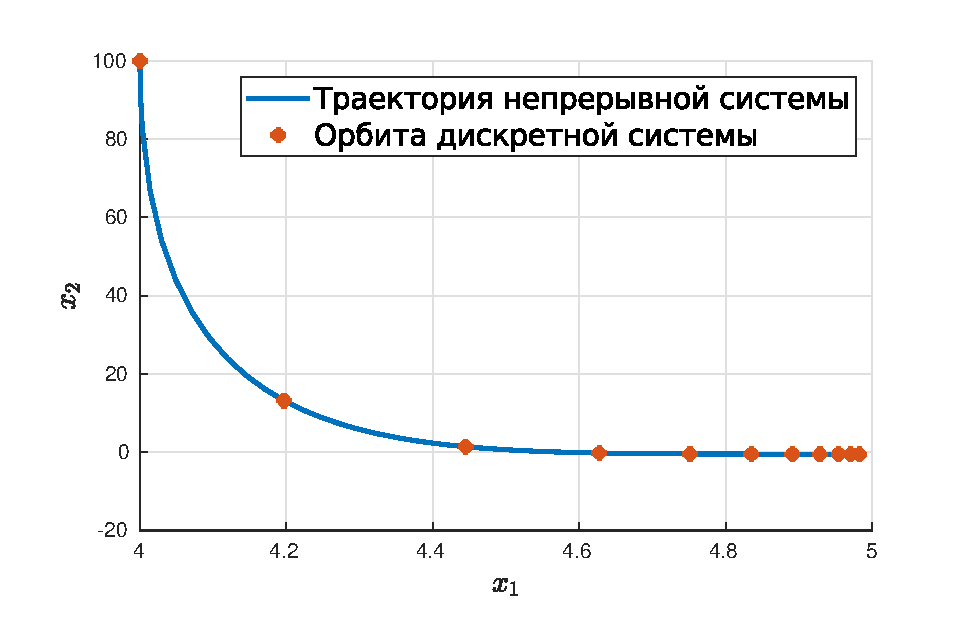
\includegraphics[width=1.15\textwidth]{content/discrete-example/cont-and-disc.eps}
                        \end{column}
                        \begin{column}{0.5\textwidth}
                                Траектория системы при передаче ей постоянного управления $u(t) \equiv 1$. 

                                \vspace{0.8cm}

                                Параметры дискретизации $\varepsilon = 0,\!2$, $h = 0,\!05$.
                        \end{column}
                \end{columns}
        \end{frame}
%%%%%%%%%%%%%%%%%%%%%%%%%%%%%%%%%%%%%%%%%%%%%%%%%%%%%%%%%%%%%%%%%%%%%%%%%%%%%%%%
        \begin{frame}{Пример}
                \center{
                        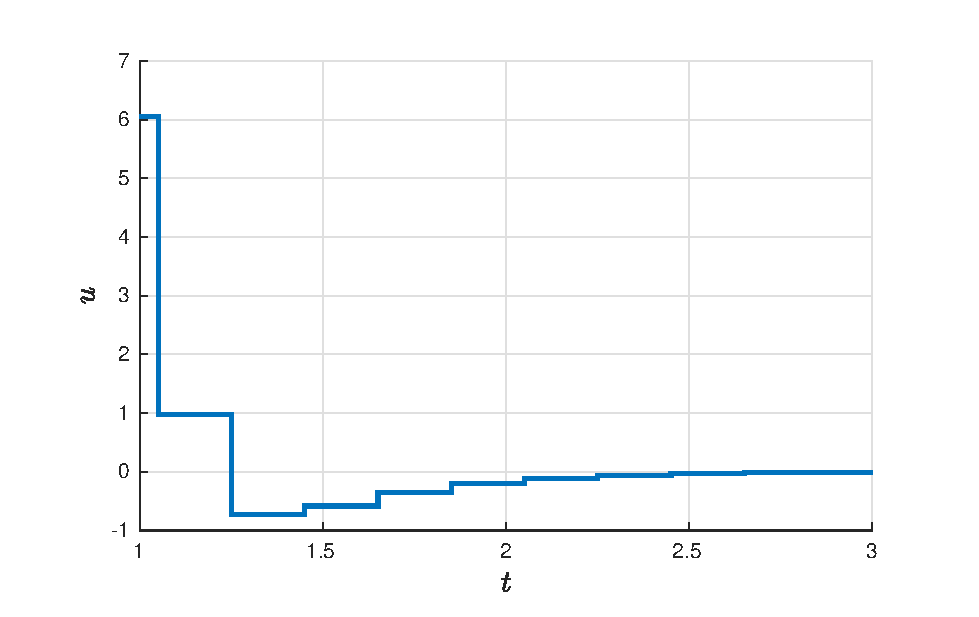
\includegraphics[width=0.8\textwidth]{content/discrete-example/control.eps}
                }
                Построенное управление на интервале $[1,\,3]$ при параметрах
                $$
                        M = \begin{pmatrix}
                1 & 0 \\
                0 & 10
                        \end{pmatrix},
                        \quad
                        N = (1),
                        \quad
                        T = \begin{pmatrix}
                1 & 0 \\
                0 & 1
                        \end{pmatrix},
                        \quad
                        x(1) = \begin{pmatrix}
                4 \\
                100
                        \end{pmatrix}.
                $$
        \end{frame}
%%%%%%%%%%%%%%%%%%%%%%%%%%%%%%%%%%%%%%%%%%%%%%%%%%%%%%%%%%%%%%%%%%%%%%%%%%%%%%%%
        \begin{frame}{Пример}
                Сравним с непрерывным решением
                \begin{columns}
                        \begin{column}{0.45\textwidth}
                                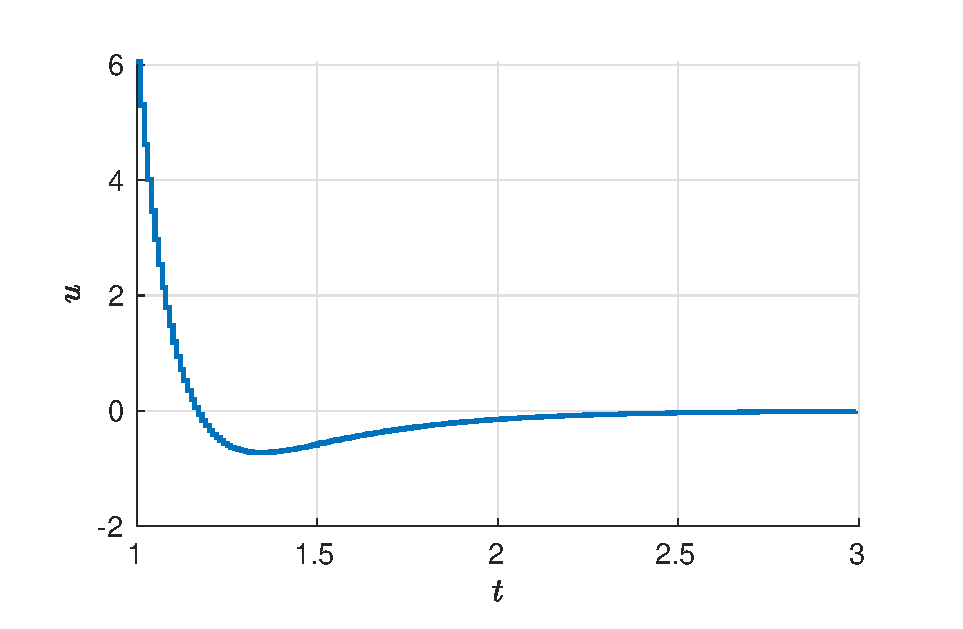
\includegraphics[width=1.15\textwidth]{content/continuous_task/example/small-control.eps}
                        \end{column}
                        \begin{column}{0.55\textwidth}
                                Управление, построенное нами.

                                \vspace{0.2cm}
                                
                                Параметры $\varepsilon = 0,\!01$, $h = 0,\!2$.

                                Значение функционала $J = 4971,\!0$.
                        \end{column}
                \end{columns}
                \begin{columns}
                        \begin{column}{0.45\textwidth}
                                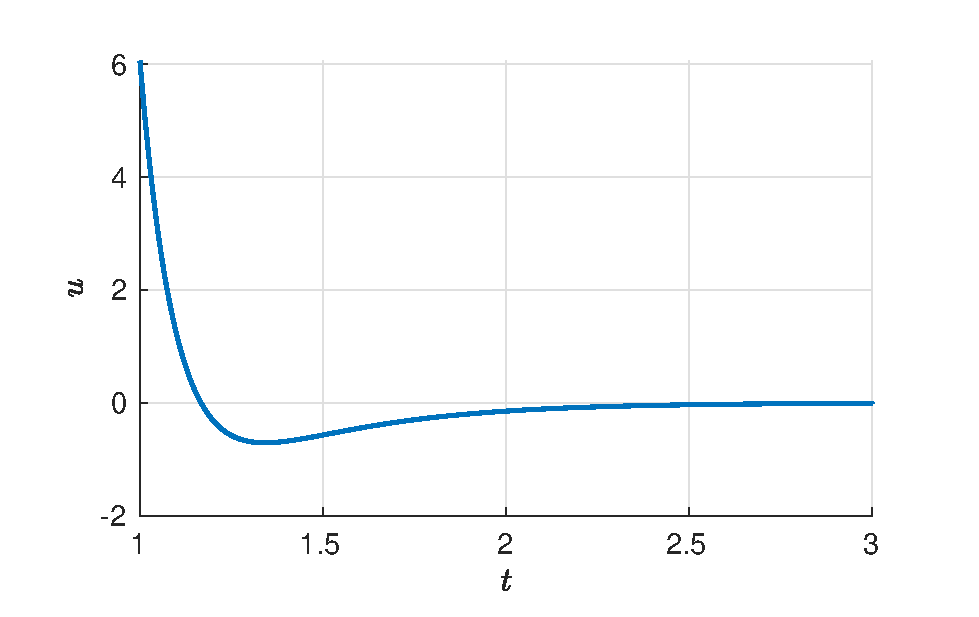
\includegraphics[width=1.15\textwidth]{content/continuous_task/example/simple-control.eps}
                        \end{column}
                        \begin{column}{0.55\textwidth}
                                Управление непрерывной системой без запаздывания.

                                \vspace{0.2cm}

                                Значение функционала $J = 4970,\!8$.
                        \end{column}
                \end{columns}
        \end{frame}
%%%%%%%%%%%%%%%%%%%%%%%%%%%%%%%%%%%%%%%%%%%%%%%%%%%%%%%%%%%%%%%%%%%%%%%%%%%%%%%%
        \begin{frame}{Планы дальнейшей работы}
                \begin{itemize}
                        \item Исследовать задачу минимизации других функционалов.
                        \item Исследовать систему с неопределенностью.
                \end{itemize}
        \end{frame}
%%%%%%%%%%%%%%%%%%%%%%%%%%%%%%%%%%%%%%%%%%%%%%%%%%%%%%%%%%%%%%%%%%%%%%%%%%%%%%%%
        \begin{frame}{Литература}
                \begin{enumerate}
                \item Беллман Р. \textit{Динамическое программирование.} М.: Изд-во иностр. лит., 1960, 400с.

                \item  Егоров А. И. \textit{Уравнения Риккати.} М.: Физматлит, 2001, 320с.

                \item Johan Nilsson. \textit{Real-Time Control Systems with Delays.} Lund Institute of Technology, 1998.

                %\item Kurzhanski A. B., Varaiya P. \textit{Systems \& Control: Foundations \& Applications.} Switzerland: Springer International Publishing, 2014.

                \item Ruba M. K. Al-Mulla Hummadi \textit{Simulation Of Optimal Speed Control For a Dc Motor Using Linear Quadratic Regulator (LQR).} Juornal of Engineering, Number 3, Volume 18 march 2012, Baghdad.
                \end{enumerate}
        \end{frame}
\end{document}